% Options for packages loaded elsewhere
\PassOptionsToPackage{unicode}{hyperref}
\PassOptionsToPackage{hyphens}{url}
%
\documentclass[
]{article}
\usepackage{amsmath,amssymb}
\usepackage{iftex}
\ifPDFTeX
  \usepackage[T1]{fontenc}
  \usepackage[utf8]{inputenc}
  \usepackage{textcomp} % provide euro and other symbols
\else % if luatex or xetex
  \usepackage{unicode-math} % this also loads fontspec
  \defaultfontfeatures{Scale=MatchLowercase}
  \defaultfontfeatures[\rmfamily]{Ligatures=TeX,Scale=1}
\fi
\usepackage{lmodern}
\ifPDFTeX\else
  % xetex/luatex font selection
\fi
% Use upquote if available, for straight quotes in verbatim environments
\IfFileExists{upquote.sty}{\usepackage{upquote}}{}
\IfFileExists{microtype.sty}{% use microtype if available
  \usepackage[]{microtype}
  \UseMicrotypeSet[protrusion]{basicmath} % disable protrusion for tt fonts
}{}
\makeatletter
\@ifundefined{KOMAClassName}{% if non-KOMA class
  \IfFileExists{parskip.sty}{%
    \usepackage{parskip}
  }{% else
    \setlength{\parindent}{0pt}
    \setlength{\parskip}{6pt plus 2pt minus 1pt}}
}{% if KOMA class
  \KOMAoptions{parskip=half}}
\makeatother
\usepackage{xcolor}
\usepackage[margin=1in]{geometry}
\usepackage{graphicx}
\makeatletter
\def\maxwidth{\ifdim\Gin@nat@width>\linewidth\linewidth\else\Gin@nat@width\fi}
\def\maxheight{\ifdim\Gin@nat@height>\textheight\textheight\else\Gin@nat@height\fi}
\makeatother
% Scale images if necessary, so that they will not overflow the page
% margins by default, and it is still possible to overwrite the defaults
% using explicit options in \includegraphics[width, height, ...]{}
\setkeys{Gin}{width=\maxwidth,height=\maxheight,keepaspectratio}
% Set default figure placement to htbp
\makeatletter
\def\fps@figure{htbp}
\makeatother
\setlength{\emergencystretch}{3em} % prevent overfull lines
\providecommand{\tightlist}{%
  \setlength{\itemsep}{0pt}\setlength{\parskip}{0pt}}
\setcounter{secnumdepth}{-\maxdimen} % remove section numbering
\ifLuaTeX
  \usepackage{selnolig}  % disable illegal ligatures
\fi
\IfFileExists{bookmark.sty}{\usepackage{bookmark}}{\usepackage{hyperref}}
\IfFileExists{xurl.sty}{\usepackage{xurl}}{} % add URL line breaks if available
\urlstyle{same}
\hypersetup{
  pdftitle={Power sim for cow nutrition},
  pdfauthor={Ed Harris},
  hidelinks,
  pdfcreator={LaTeX via pandoc}}

\title{Power sim for cow nutrition}
\author{Ed Harris}
\date{2023-06-22}

\begin{document}
\maketitle

\hypertarget{summary}{%
\subsection{Summary}\label{summary}}

The goal here was to simulate power for several sample size scenarios
for a 4x4 Latin Square design. A balanced Latin sq. design would
typically have an equal replicate size for each cohort (e.g.~n=8 {[}or
another multiple of 4{]}, with 2 individuals per cohort with 4 cohorts
in a 4x4 design). However only 7 or 6 subjects are available. The
question is how does this affect power? I assumed the analysis to be a
linear mixed effects model (as an alternative to ANOVA for fully
balanced design), with individual \texttt{Cow} as a random effect and
\texttt{Diet} treatment (4 levels) as a fixed effect.

~

\(y_t = \beta_0 + \boldsymbol{B}_1 * (Diet) + (b_s)_t + \epsilon_t\)

~

where \(\beta_0\) is the mean response, \(\boldsymbol{B}_1\) is the
matrix of Diet-specific effect estimates, \(b_s\) is the random effect
of subject \(s\), and \(\epsilon_t\) is the assumed-Gaussian residual
error.

~

Power analysis for linear mixed effects models can be challenging; here
a simulation approach was used (e.g., see Kumle et al.~2021). Pilot data
were provided for two dependent variables, \texttt{pH} and
\texttt{Ammonia}, and parameter for the simulation model were estimated
based on them to simulate statistical power for detecting a treatment
effect of \texttt{Diet} for \(n=\) 8, 7 or 6 subjects. For each model,
500 datasets were simulated for each sample size, and each sample size
was modeled for the observed pilot variance, for +10\% observed pilot
variance and for -10\% observed variance (\texttt{med}, \texttt{high}
and \texttt{low}, respectively). The \texttt{\{lme4\}} package (Bates et
al.~2015) was used for the linear mixed effects modelling using R v
4.3.0 (R Core Team 2023). The pilot data only contained three feed
treatments, so the four treatment experiment was modeled using the
observed treatment extremes, with an extrapolated monotonic increase in
effect size for the two other treatments within the range of extremes.

~

Table 1. The parameter sets used for power simulations.

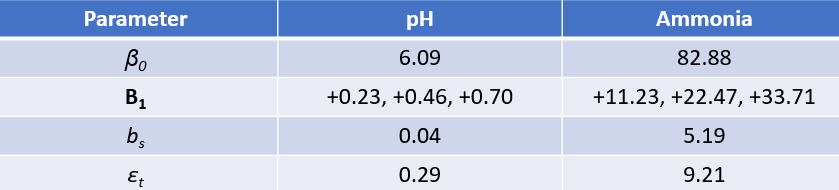
\includegraphics{figs/parameters.png}

\newpage

\hypertarget{results}{%
\subsection{Results}\label{results}}

Figure 1. Panels \texttt{A} and \texttt{B} contain the power analysis
results for pH and Ammonia, respectively. The red horizontal dashed line
indicates 80\% power. Each solid line represents a variance value across
n = 6,7 or 8 cows. The purple dot indicates expected power for the pilot
data parameterised variance (\texttt{med}) for n = 7 cows. Panels
\texttt{C} and \texttt{D} show pilot data for \texttt{pH} and
\texttt{Ammonia}, respectively. Each line represents a different
\texttt{Cow}.

~

The expected power for n=7 for \texttt{pH} is slightly below 80\% power,
while the expected power for all replicate sizes are far above 80\%
power for \texttt{Ammonia.}

~

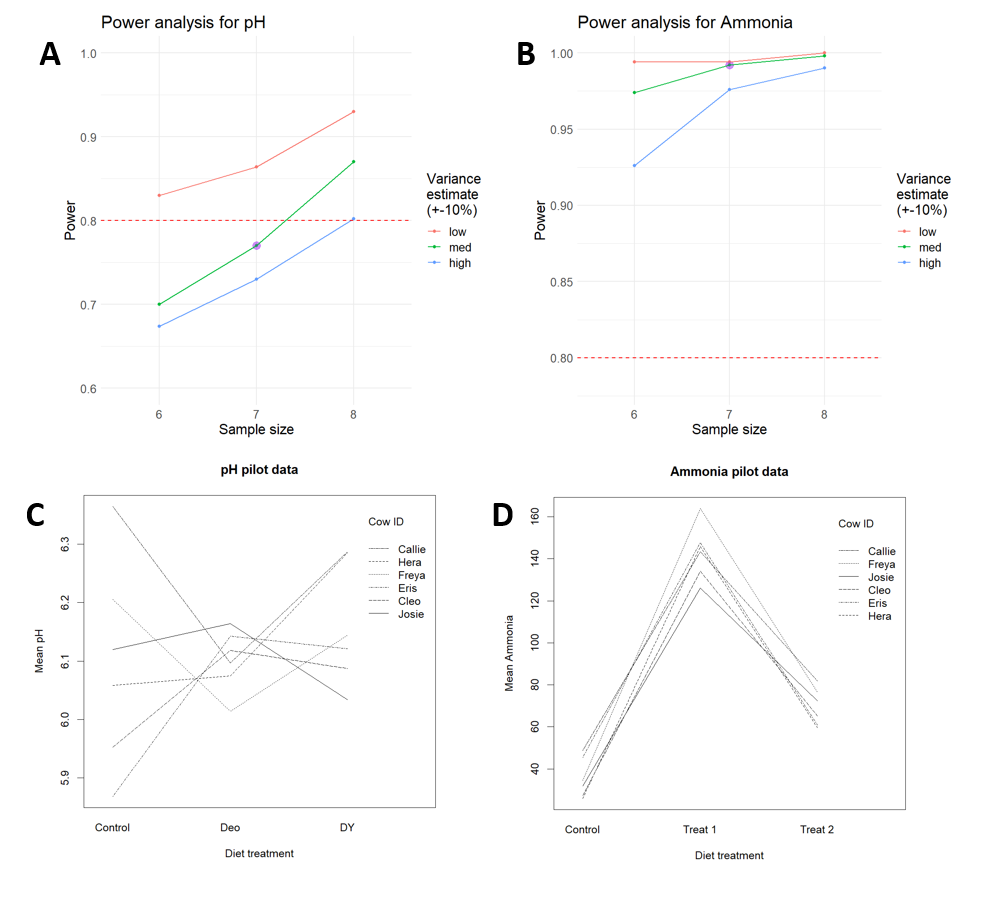
\includegraphics{figs/Fig1.png}

\newpage

\hypertarget{references}{%
\subsection{References}\label{references}}

Bates, D., Maechler, M., Bolker, B., Walker, S. 2015. Fitting Linear
Mixed-Effects Models Using lme4. Journal of Statistical Software, 67(1),
1-48. \url{doi:10.18637/jss.v067.i01}.

Kumle, L., Võ, M.L.-H., Draschkow, D., 2021. Estimating power in
(generalized) linear mixed models: An open introduction and tutorial in
R. Behav Res 53, 2528--2543.
\url{https://doi.org/10.3758/s13428-021-01546-0}

R Core Team 2023. R: A Language and Environment for Statistical
Computing. R Foundation for Statistical Computing, Vienna, Austria.
\url{https://www.R-project.org/}.

\end{document}
